\section{Parte Frontal} 

A parte frontal da estrutura, mostrada na Figura \ref{partedafrente}, comporta a roda dianteira da bicicleta e é responsável pela elevação e descida da plataforma dando a sensação de um terreno com variação de altura para que o usuário tenha uma experiência mais imersiva ao ambiente virtual.

    \begin{center}
        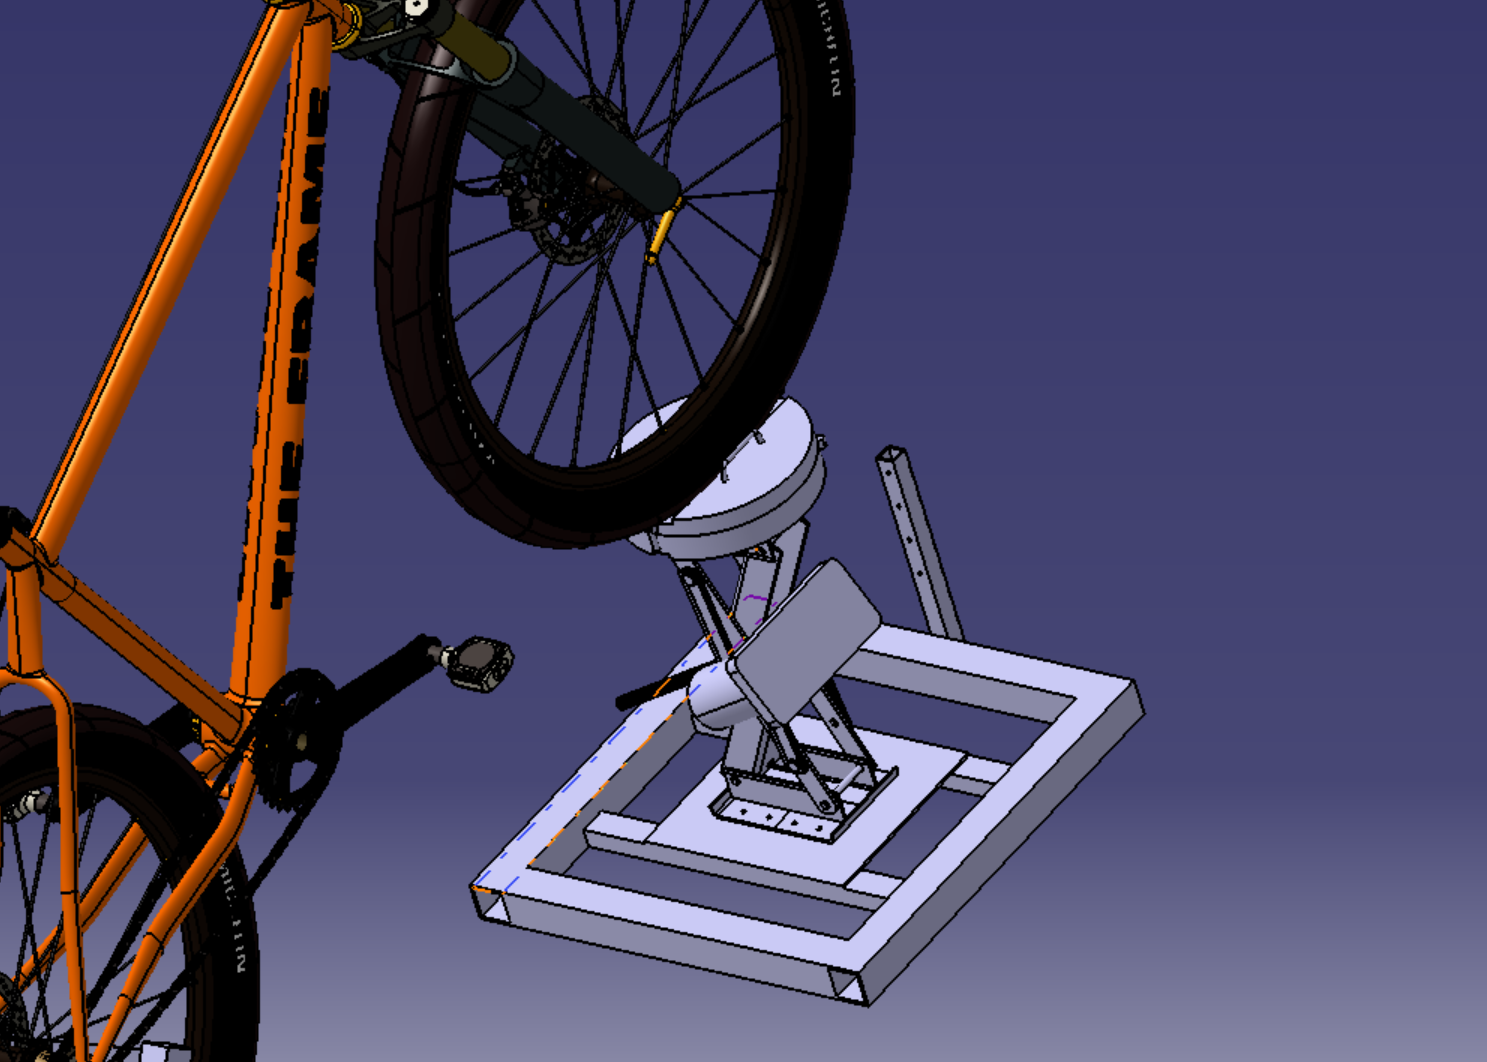
\includegraphics[scale=0.4]{figuras/partedafrente.png}
        \captionof{figure}{CAD da estrutura dianteira}
        \label{partedafrente}
    \end{center}
    
    % Foto real estrutura dianteira

    Como anteriormente definido a esta parte fronta comporta:
    \begin{itemize}
        \item Macaco elétrico - sincronizado com o ambiente virtual para elevar e descer a bicicleta enquanto suporta o peso do usuário e da estrutura complementar.

        \item Mesa giratória – Usinada para ser acoplada ao macaco e suportar os esforços de peso, composta por 3 peças mecânicas;
            \begin{itemize}
                \item Base da mesa giratória – Acoplada a base do macaco e onde ocorre o acoplamento ‘fêmea’ do rolamento e furo para abrigar potenciômetro;
                \item Rolamento;
                \item Mesa giratória em si – Acoplada como "macho" no rolamento e sustentando a roda dando segurança e permitindo o giro do guidão controlando jogo
            \end{itemize}
    \end{itemize}    


\subsection{Mesa Giratória}

    \begin{center}
        \includegraphics[scale=0.7]{figuras/acoplamento_frontal}
        \captionof{figure}{Esquema de acoplamento da parte frontal}
        \label{acoplamento_frontal}
    \end{center}
    
    \begin{center}
        \includegraphics[scale=0.7]{figuras/acoplamento_frontal_2}
        \captionof{figure}{Outra vista do esquema de acoplamento}
        \label{acoplamento_frontal_2}
    \end{center}


    Tendo em vista o planejamento da montagem final, apresentadas nas Figuras acimas, começou-se o dimensionamento das peças a serem fabricadas.

    Para calcular os esforços para as simulações foram feitos os cálculos abaixo

    \begin{center}
        \includegraphics[scale=0.7]{figuras/analise_corpos_livres}
        \captionof{figure}{Análise de Corpos Livres}
        \label{analise_corpos_livres}
    \end{center}

    Como não há um padrão para distância entre os eixos e no centro de massa, medimos as distâncias da bicicleta que usamos nos desenhos em CAD. Com elas, utilizou-se conhecimentos básicos em estática para calcular a força resultante em cada roda. 

    Utilizando como momento nulo o centro da roda traseira e considerando que toda a plataforma mais o usuário gerem uma força de 1000 N, temos que:

\begin{equation}\label{eq290}
    \sum F = 0 
\end{equation}

 \begin{equation}\label{eq291}
    F2 \cdot 1110,295 - 1000 \cdot 479,176 = 0 
\end{equation}

 \begin{equation}\label{eq292}
    F2 = ~431,6 N
\end{equation}

 \begin{equation}\label{eq293}
    F1 =~ 568,4 N
\end{equation}

    Como a bicicleta varia sua inclinação em um ângulo muito pequeno, podemos aproximar para essa força em todo o percurso.

    Com as forças definidas foram feitas as simulações nas duas peças a serem usinadas no software ANSYS para avaliação dos resultados, validação e posterior usinagem.

    Para a parte superior da mesa foram feitas tais simulações:

     \begin{center}
        \includegraphics[scale=0.7]{figuras/sim_estatica_1}
        \captionof{figure}{Simulação estática estrutural – Tensão elástica equivalente}
        \label{sim_estatica_1}
    \end{center}
    
     \begin{center}
        \includegraphics[scale=0.7]{figuras/stress_1}
        \captionof{figure}{Stress equivalente com Tensão de escoamento da mesa superior}
        \label{stress_1}
    \end{center}

     \begin{center}
        \includegraphics[scale=0.7]{figuras/fator_seguranca_1}
        \captionof{figure}{Fator de segurança da mesa superior}
        \label{fator_seguranca_1}
    \end{center}

     \begin{center}
        \includegraphics[scale=0.7]{figuras/vida_util_1}
        \captionof{figure}{Vida útil da mesa giratória}
        \label{vida_util_1}
    \end{center}

    Como pode ser observado, todos os testes validam a peça para fabricação:

    \begin{itemize}
        \item A Figura \ref{sim_estatica_1} mostra a deformação máxima (em mm) que a peça sofre com a carga aplicada e esta deformação é quase nula;
        \item A Figura \ref{stress_1}  mostra a tensão de escoamento que o material alcança (3,1662 MPa), sendo muito inferior a tensão de escoamento do aço 1045 (310 Mpa);
        \item A Figura \ref{fator_seguranca_1} mostra o Fator de segurança da peça pelas condições de contorno, sendo esse fator igual a 15;
        \item A Figura \ref{vida_util_1} mostra a vida útil da peça tendo como resultado uma peça com vida útil muito grande.
    \end{itemize}
  
    Conclui-se que essas peças são validadas para usinagem pois suportam com segurança os esforços nela aplicado. É possível observar que é uma peça superdimensionada, mas como um dos objetivos do projeto é a segurança do usuário e o macaco suporta o peso este fato é descartado. Seu desenho técnico se encontra no final deste documento, no anexo \ref{anexo_megi_superior}.

    Para a base da mesa giratória foram feitas tais simulações:

    \begin{center}
        \includegraphics[scale=0.7]{figuras/modal_corpo_livre_1}
        \captionof{figure}{Modal de corpo livre - Deformação total }
        \label{modal_corpo_livre_1}
    \end{center}

    \begin{center}
        \includegraphics[scale=0.7]{figuras/ressonancia_1}
        \captionof{figure}{Módulos de vibração de ressonância da peça}
        \label{ressonancia_1}
    \end{center}
    
    \begin{center}
        \includegraphics[scale=0.7]{figuras/sim_estatica_2}
        \captionof{figure}{Simulação estática estrutural – Tensão elástica equivalente}
        \label{sim_estatica_2}
    \end{center}
    
    \begin{center}
        \includegraphics[scale=0.7]{figuras/stress_2}
        \captionof{figure}{Stress equivalente com Tensão de escoamento}
        \label{stress_2}
    \end{center}
    
    \begin{center}
        \includegraphics[scale=0.7]{figuras/fator_seguranca_2}
        \captionof{figure}{Fator de Segurança}
        \label{fator_seguranca_2}
    \end{center}
    
    \begin{center}
        \includegraphics[scale=0.7]{figuras/vida_util_2}
        \captionof{figure}{Vida útil}
        \label{vida_util_2}
    \end{center}

    Como pode ser observado, todos os testes também validam a peça para fabricação:
    \begin{itemize}
        \item A Figura \ref{modal_corpo_livre_1} e  \ref{ressonancia_1} mostram os resultados da análise modal de corpo livre mostrando a deformação total que as frequências causariam, que novamente são quase nulas, e as valores os quais a peça entra em ressonância, não tendo impacto pois a frequência gerada pelo macaco não conflita com nenhum dos valores atingidos
        \item A Figura \ref{sim_estatica_2} mostra a deformação máxima (em mm) que a peça sofre com a carga aplicada e esta deformação é quase nula;
        \item A Figura \ref{stress_2} mostra a tensão de escoamento que o material alcança (1,4389 MPa), sendo também muito inferior a tensão de escoamento do aço 1045 (310 Mpa);
        \item A Figura \ref{fator_seguranca_2} mostra o Fator de segurança da peça pelas condições de contorno, sendo esse fator também igual a 15;
        \item A Figura \ref{vida_util_2} mostra a vida útil da peça tendo como resultado uma peça com vida útil muito grande.
    \end{itemize}

    \begin{center}
        \includegraphics[scale=0.4]{figuras/mesa_giratoria_1}
        \captionof{figure}{Mesa giratória usinada}
        \label{mesa_giratoria_1}
    \end{center}

    Os resultados apresentados também a validam para usinagem pois nas simulações são suportados todos os esforços exigidos e nenhum fator oferece risco algum ao usuário. Esta peça também é superdimensionada mas isso não oferece nenhuma perda ao projeto e o resultado final. Para detalhes técnicos da geometria da peça, o desenho técnico se encontra no anexo \ref{anexo_megi_inferior}.
    
    Para a versão final foram colocados suportes para uma cinta para fixar a roda dianteira da bicicleta, como mostrado na figura abaixo. Algumas outras alterações foram feitas que serão explicadas na parte de integração com outras áreas, a sessão \ref{secao.integracao}.
    
    % foto real e atual da mesa giratória

\subsection{Macaco de Elevação}

  Com a exigência de fazer a elevação durante a simulação, foi projetado a utilização de um macaco que esticaria ao total 230 mm. Isso dá em torno de 6 graus de subida e 6 de descida. O motor que necessário para gerar a subida e descida da plataforma tem elevada dimensões e peso bem maior que a do macaco tornando a fixação do motor ao macaco complexa, por sugestão do professor Rhander, escolheu-se comprar um macaco elétrico, da figura \ref{macaco_eletrico_1}, pois é uma solução viável dentro do orçamento disponível.

    \begin{center}
        \includegraphics[scale=0.5]{figuras/macaco_eletrico_1}
        \captionof{figure}{Macaco com motor elétrico}
        \label{macaco_eletrico_1}
    \end{center}    

\subsection{Integração Parte Dianteira}
  Para a fase final do projeto dessa parte, foram feitas as seguintes ações de integração da estrutura:
  \begin{itemize}
        \item Construção de uma estrutura de suporte dianteiro para melhor sustentar toda a estrutura na parte frontal.
        \item Parafusar o macaco nesta estrutura.
        \item Parafusar o macaco na base da mesa giratória.
        \item Fazer uma estrutura de cinta para fixar a roda na mesa giratória.
    \end{itemize}
    
    \begin{center}
        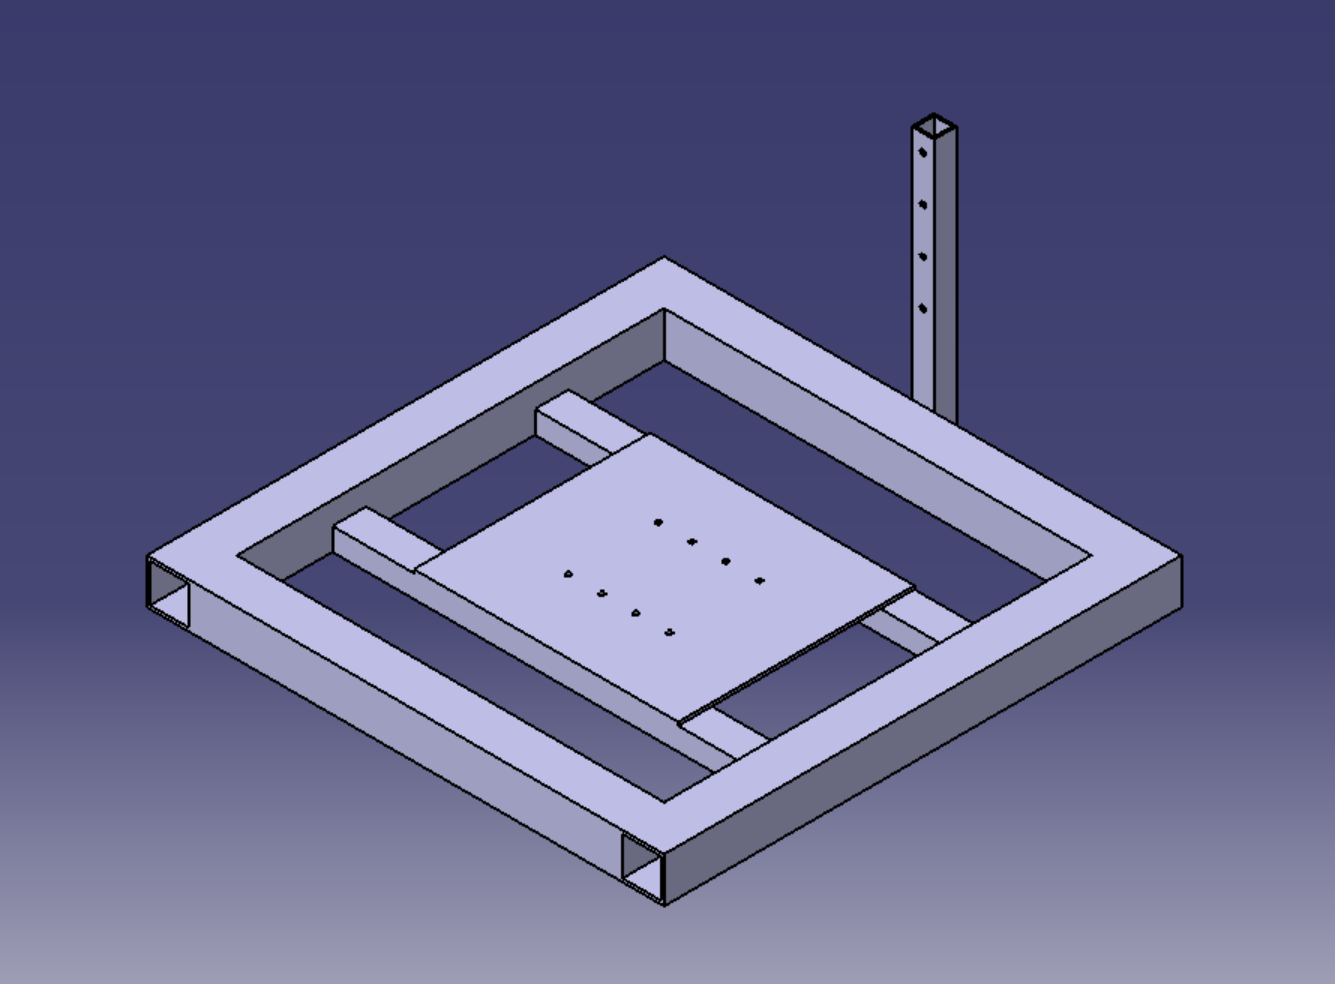
\includegraphics[scale=0.5]{figuras/Base_dianteira}
        \captionof{figure}{Estrutura de suporte dianteiro}
        \label{base_dianteira}
    \end{center}  

    Na Figura \ref{base_dianteira} é mostrado a estrutura feita para dar maior estabilidade em um sistema que tem subidas e descidas. Ainda foi aproveitado essa estrutura para atender ao requisito pedido pelos professores de criar uma resistência ao girar o guidão. A solução foi fazer alguns pontos para fixar algumas molas que serão fixadas na mesa giratória, aumentando conforme o giro no guidão. No anexo \ref{anexo_base_frontal}, encontra-se o desenho técnico dessa peça.
    
        \begin{center}
        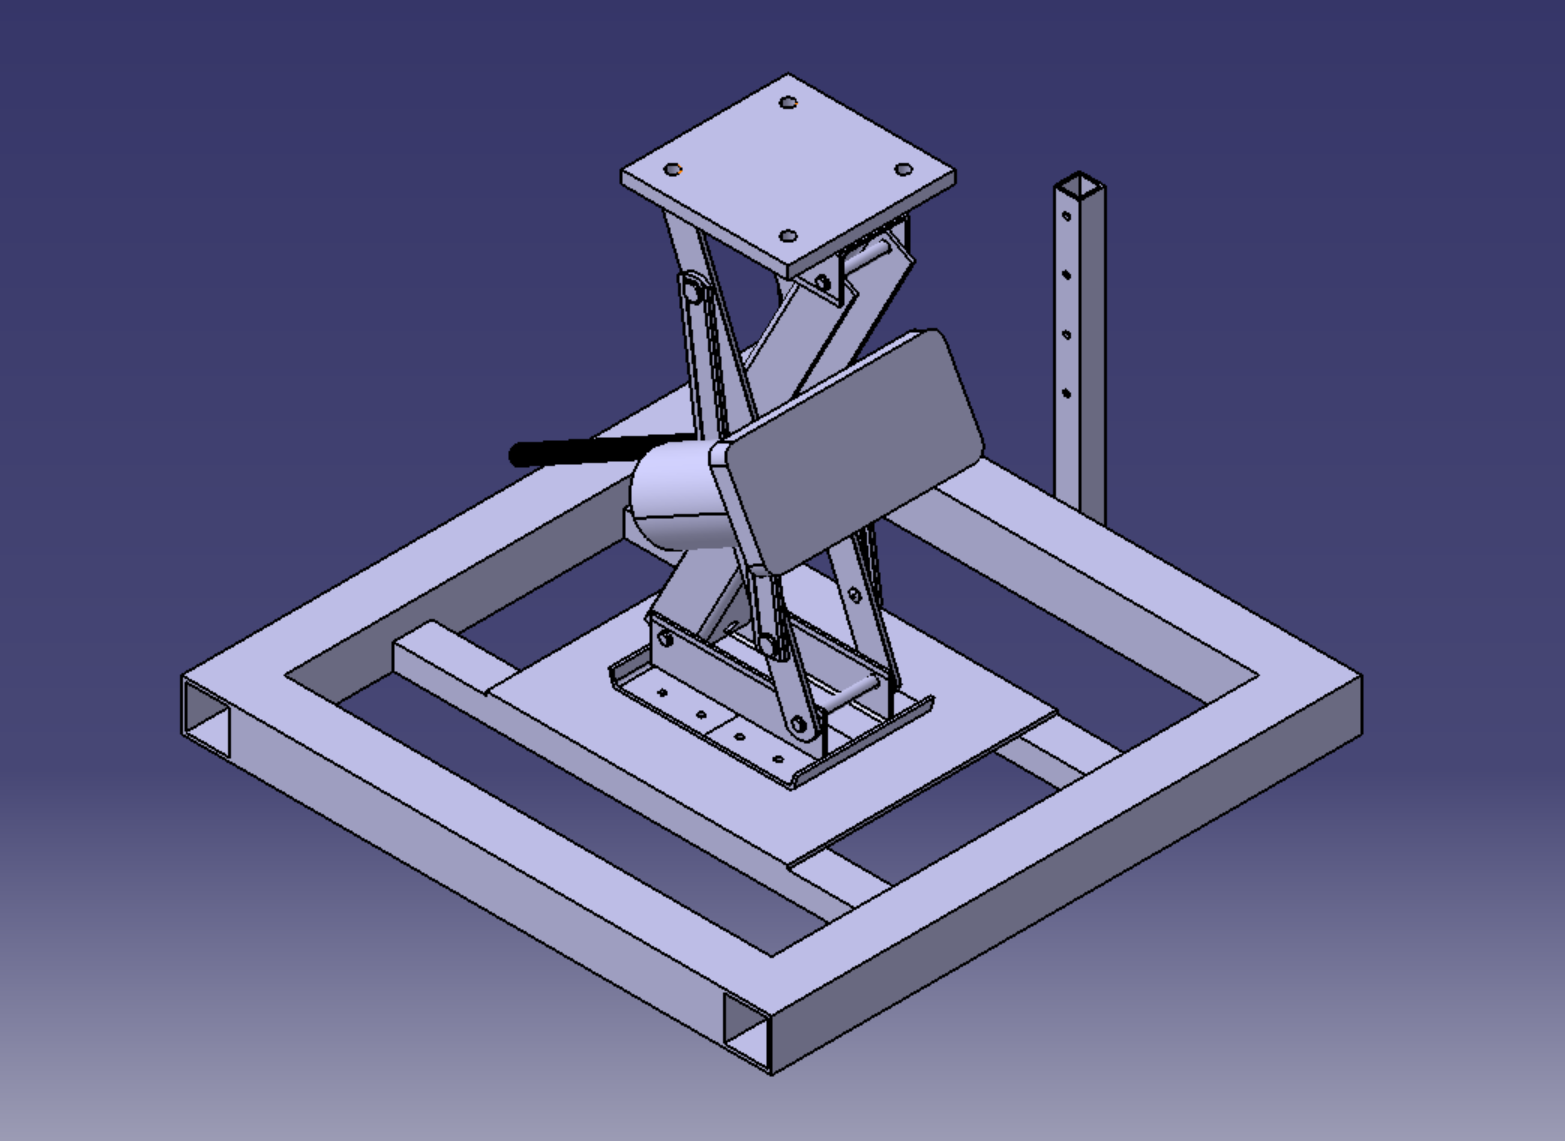
\includegraphics[scale=0.5]{figuras/Base_dianteira_macaco}
        \captionof{figure}{Estrutura de suporte dianteiro com o macaco integrado}
        \label{base_dianteira_macaco}
    \end{center}  
    
    A sequência apresentada na figura acima apresenta a integração entre a estrutura de suporte dianteiro e o macaco por meio de parafusos. Há ainda visível uma estrutura soldada em cima do macaco para facilitar a integração com a base da mesa giratória, apresentada na imagem abaixo.
    
            \begin{center}
        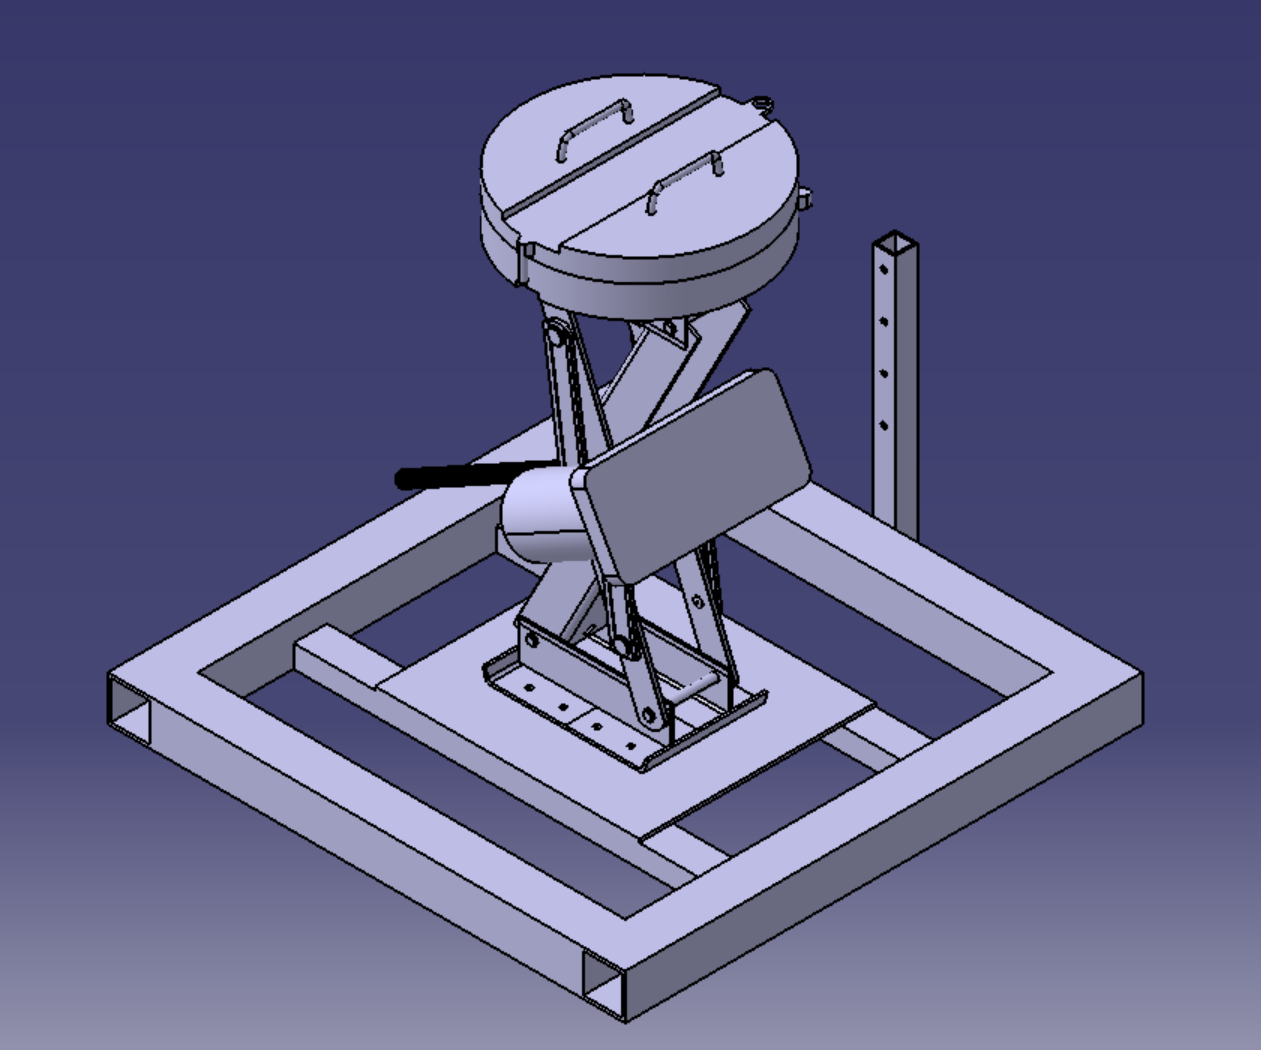
\includegraphics[scale=0.5]{figuras/Base_dianteira_macaco_mesagiratoria}
        \captionof{figure}{Parte dianteria completa}
        \label{Base_dianteira_macaco_ mesagiratoria}
    \end{center}  

    Assim é possível parafusar a base da mesa giratória no macaco, integrando os sistemas da parte frontal. Alguns detalhes particulares da integração com outras áreas serão apresentadas na sessão \ref{secao.integracao}. Abaixo vê-se a foto real da parte dianteira para comparação.
    
    % Foto real parte dianteira

\section{Parte Traseira}
    A parte traseira da plataforma, na Figura \ref{parte_traseira_1} representada, garante a interação com a realidade aumentada através de sensores de velocidade, controle de peso na pedalada para simular subida e geração de energia. É adaptável a diferentes tamanhos de bicicleta.
 
    \begin{center}
        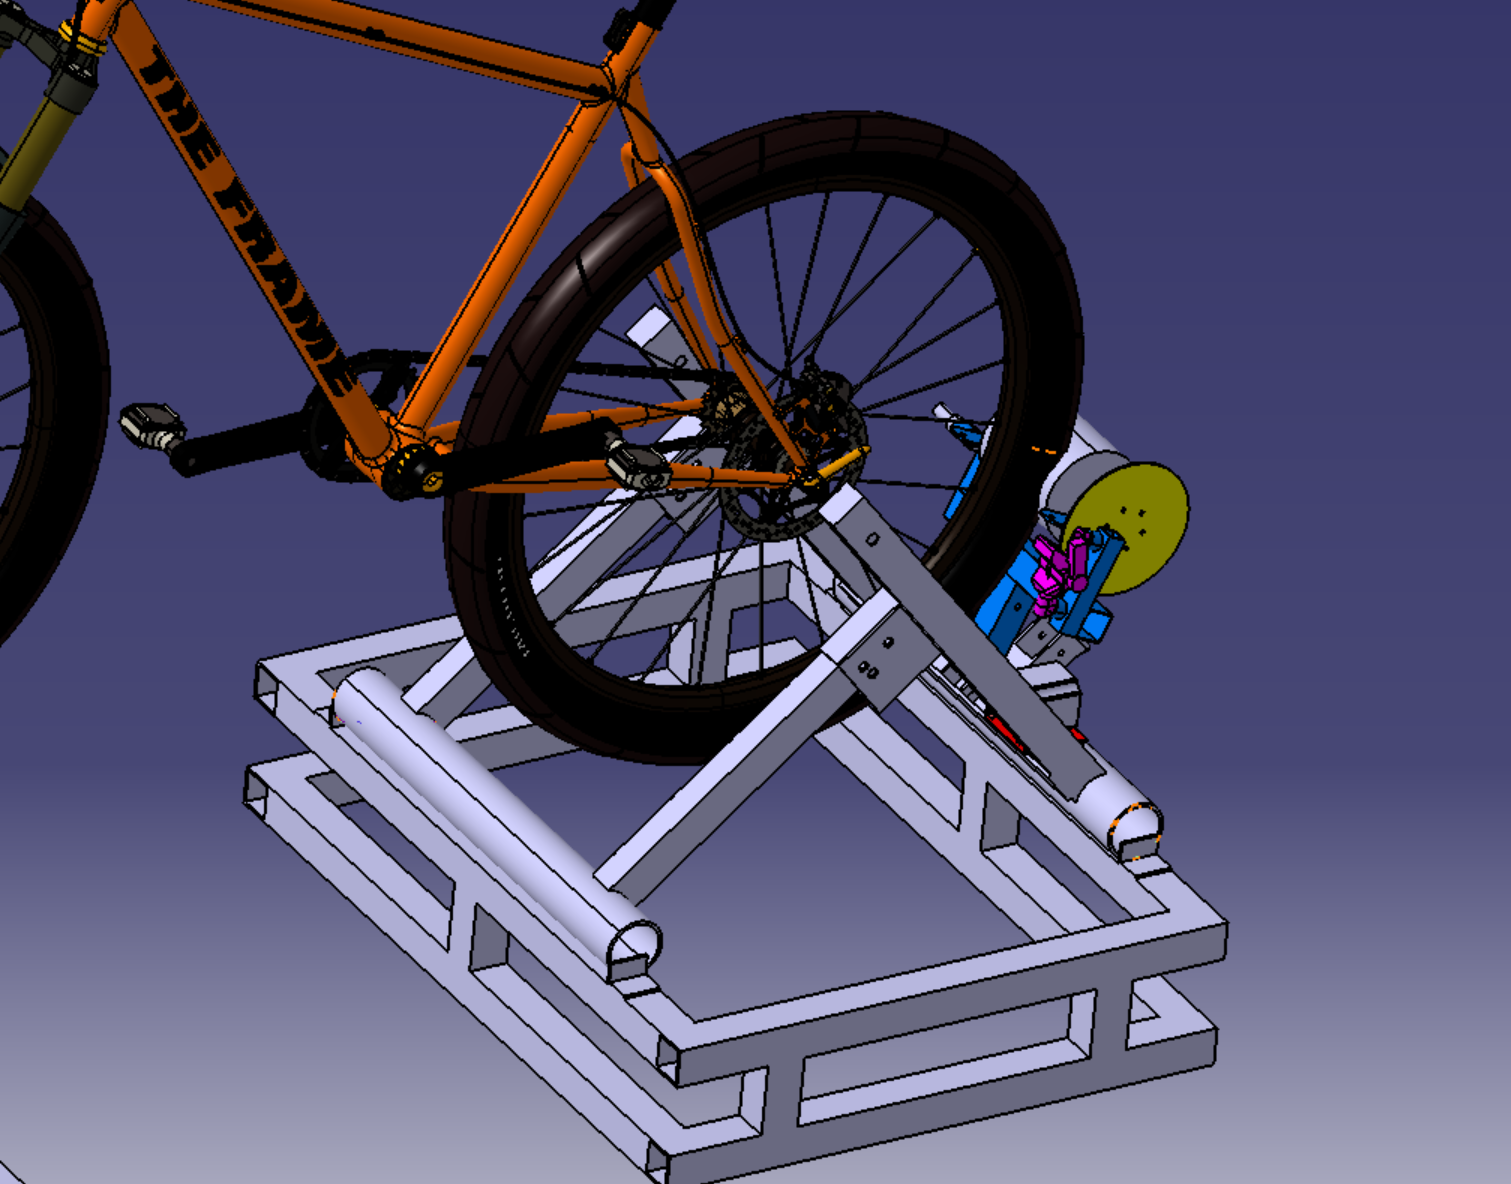
\includegraphics[scale=0.5]{figuras/parte_traseira}
        \captionof{figure}{CAD da parte traseira}
        \label{parte_traseira_1}
    \end{center}  

    % Foto real da parte traseira

   Algumas peças foram adquiridos de um projeto antigo no galpão que usava para fins semelhantes. Adaptado a ele, foram projetados o suporte do freio para controle do peso da pedalada, o suporte para o sensor RPM e estrutura de suporte traseiro para colocar a roda traseira na altura certa para a simulação, cuja detalhe técnico se encontra no anexo \ref{anexo_base_traseira}. Após tornarem-se operacional, as peças antigas foram reajustados e pintadas.

\subsection{Cavalete de sustentação}

    A estrutura traseira comporta a roda traseira da bicicleta, acoplando-as por fusos com um acoplador nas pontas que encaixa na bicicleta exatamente no eixo da roda. Essa estrutura tem como objetivo sustentar a bicicleta e comportar o rolete traseiro onde haverá o sistema de controle de peso para simulação de subida.

    Como anteriormente definido a esta parte traseira comporta:
    \begin{itemize}
        \item Duas peças que juntas se tornam um cavalete.
    \end{itemize}
    
    \begin{center}
        \includegraphics[scale=0.3]{figuras/esquema_traseira_1}
        \captionof{figure}{Esquema estrutura parte traseira}
        \label{esquema_traseira_1}
    \end{center}    

    \begin{center}
        \includegraphics[scale=0.5]{figuras/parte_traseira_2}
        \captionof{figure}{Esquema estrutura completa de acoplamento parte traseira.}
        \label{parte_traseira_2}
    \end{center}        
   
    \begin{center}
        \includegraphics[scale=0.5]{figuras/acoplamento_est_1}
        \captionof{figure}{Acoplamento estrutural em uma bicicleta.}
        \label{acoplamento_est_1}
    \end{center}      
  
    Para calcular os esforços para as simulações, foram usados os cálculos apresentados na figura \ref{analise_corpos_livres} que analisaram os esforços em corpos livres. Para os casos abaixo foram utilizados uma força de 2200 N para aumentar o fator de segurança, a fim de levar em conta uma situação extrema de uso da estrutura. Ao fazer a decomposição dos vetores, essas forças foram distribuídas nos eixos X e Z (de acordo com o sistema de referência do ANSYS), conforme mostrado nas Figuras \ref{forcas_1} e \ref{forcas_2}.

    \begin{center}
        \includegraphics[scale=0.7]{figuras/forcas_1}
        \captionof{figure}{Aplicação das forças}
        \label{forcas_1}
    \end{center}   
    
    \begin{center}
        \includegraphics[scale=0.7]{figuras/forcas_2}
        \captionof{figure}{Aplicação das forças em escala aumentada}
        \label{forcas_2}
    \end{center}  
 
    Com as forças definidas foram feitas as simulações no cavalete pois ele é o componente estrutural e que sustenta a maior carga, sendo ela a junção do peso da bicicleta e do jogador e suas energias consequentes.
 
    Para a parte traseira foram divididas em 2 partes:
    \begin{itemize}
        \item Simulações na peça sem rolo do cavalete – Peça 1.
        \item Simulações na peça com rolo do cavalete – Peça 2.
    \end{itemize}
 
    \begin{center}
        \includegraphics[scale=0.7]{figuras/sim_estatica_3}
        \captionof{figure}{Simulação estática peça 1 – Tensão elástica equivalente}
        \label{sim_estatica_3}
    \end{center}
    
    \begin{center}
        \includegraphics[scale=0.7]{figuras/stress_3}
        \captionof{figure}{Stress equivalente com Tensão de escoamento da peça 1}
        \label{stress_3}
    \end{center}
    
    \begin{center}
        \includegraphics[scale=0.7]{figuras/deformacao_1}
        \captionof{figure}{Total deformação da peça 1}
        \label{deformacao_1}
    \end{center}

    \begin{center}
        \includegraphics[scale=0.7]{figuras/fator_seguranca_3}
        \captionof{figure}{Fator de Segurança da peça 1}
        \label{fator_seguranca_3}
    \end{center}
    
    \begin{center}
        \includegraphics[scale=0.7]{figuras/vida_util_3}
        \captionof{figure}{Vida útil da peça 1}
        \label{vida_util_3}
    \end{center}

    \begin{center}
        \includegraphics[scale=0.7]{figuras/vibracao_1}
        \captionof{figure}{Modos de vibração de ressonância da peça 1}
        \label{vibracao_1}
    \end{center}    
 
    Como pode ser observado, todos os testes validam a peça para fabricação:
    \begin{itemize}
        \item A figura \ref{sim_estatica_3} mostra a deformação elástica (em mm) que a peça 1 sofre com a carga aplicada, esta deformação é considerada nula;
        \item A figura \ref{stress_3} mostra a tensão de escoamento que o material da peça 1 alcança (75,91 MPa), sendo muito inferior a tensão de escoamento do aço 1045 (310 Mpa);
        \item A figura \ref{deformacao_1} mostra a deformação total da peça 1, considerada nula.
        \item A figura \ref{fator_seguranca_3} mostra o Fator de segurança da peça 1 pelas condições de contorno, sendo esse fator igual a 15;
        \item A figura \ref{vida_util_3} mostra a vida útil da peça 1 tendo como resultado uma peça com vida útil muito grande.
        \item A figura \ref{vibracao_1} mostra os módulos de vibração da peça 1, vemos que os 6 primeiros modos de vibração são considerados nulos, para que a faça com que a estrutura entre em ressonância é necessário chegar ao sétimo modo de vibração de 229,46 Hz, sendo que para a aplicação desta estrutura tal frequência jamais será alcançada.
    \end{itemize}
    
    A peças 1 suporta com segurança os esforços nela aplicado. Para ver o desenho técnico dessa peça, ver anexo \ref{anexo_pe_sem_rolo}.
 
    Para a peça 2 foram feitas tais simulações:
 

    \begin{center}
        \includegraphics[scale=0.7]{figuras/sim_estatica_4}
        \captionof{figure}{Simulação estática peça 2 – Tensão elástica equivalente}
        \label{sim_estatica_4}
    \end{center}
    
    \begin{center}
        \includegraphics[scale=0.7]{figuras/stress_4}
        \captionof{figure}{Stress equivalente com Tensão de escoamento da peça 2}
        \label{stress_4}
    \end{center}
  
    \begin{center}
        \includegraphics[scale=0.7]{figuras/deformacao_2}
        \captionof{figure}{Modal de corpo livre - deformação total da peça 2}
        \label{deformacao_2}
    \end{center}

    \begin{center}
        \includegraphics[scale=0.7]{figuras/fator_seguranca_4}
        \captionof{figure}{Fator de Segurança da peça 2}
        \label{fator_seguranca_4}
    \end{center}
    
    \begin{center}
        \includegraphics[scale=0.7]{figuras/vida_util_4}
        \captionof{figure}{Vida útil da peça 2}
        \label{vida_util_4}
    \end{center}

    \begin{center}
        \includegraphics[scale=0.7]{figuras/vibracao_2}
        \captionof{figure}{Modos de vibração de ressonância da peça 2}
        \label{vibracao_2}
    \end{center}    

    Como pode ser observado, todos os testes também validam a peça para fabricação:
 
    \begin{itemize}
        \item A figura \ref{sim_estatica_4} mostra a deformação elástica (em mm) que a peça 2 sofre com a carga aplicada, esta deformação é considerada nula;
        \item A figura \ref{stress_4} mostra a tensão de escoamento que a peça 2 alcança (141,39 MPa), sendo também muito inferior a tensão de escoamento do aço 1045 (310 Mpa);
        \item A figura \ref{deformacao_2} mostra a deformação total da peça 2, considerada mínima.
        \item A figura \ref{fator_seguranca_4} mostra o Fator de segurança da peça 2 pelas condições de contorno, sendo esse fator também igual a 15;
        \item A figura \ref{vida_util_4} mostra a vida útil da peça 2 tendo como resultado uma peça com vida útil muito grande.
        \item Assim como a peça 1 a peça 2 possui os 6 primeiros modos e para chegar na frequência natural da peça seria necessário alcançar 2264 Hz, inalcançável considerando a sua aplicação
    \end{itemize}

A peça 2 também está válida para o uso. No anexo \ref{anexo_pe_com_rolo}, é possível encontrar o desenho técnico desse componente.

\subsection{Estrutura do freio}

A estrutura do freio Figura \ref{esq_suporte_rolo_1} e \ref{esq_suporte_rolo_2}, fica acoplado na estrutura traseira e suporta o rolo.
 
    \begin{center}
        \includegraphics[scale=0.5]{figuras/esq_suporte_rolo_1}
        \captionof{figure}{Esquema estrutura parte traseira com suporte do rolo}
        \label{esq_suporte_rolo_1}
    \end{center} 
 
    \begin{center}
        \includegraphics[scale=0.5]{figuras/esq_suporte_rolo_2}
        \captionof{figure}{Esquema estrutura completa de acoplamento parte traseira.}
        \label{esq_suporte_rolo_2}
    \end{center}
 
Para calcular os esforços para as simulações, foram usados os cálculos apresentados na Figura \ref{analise_corpos_livres}.  Foi utilizado a força total aplicada na estrutura traseira nos dois suportes do rolo e dividida simultaneamente para a superfície de contado do rolamento em vermelho na Figura \ref{forcas_3}.

    \begin{center}
        \includegraphics[scale=0.5]{figuras/forcas_3}
        \captionof{figure}{Aplicação das forças na estrutura.}
        \label{forcas_3}
    \end{center}
    
Com as forças definidas foram feitas as simulações no suporte.
    \begin{center}
        \includegraphics[scale=0.5]{figuras/sim_estatica_5}
        \captionof{figure}{Simulação estática do suporte – Tensão elástica equivalente}
        \label{sim_estatica_5}
    \end{center} 
    
     \begin{center}
        \includegraphics[scale=0.7]{figuras/stress_5}
        \captionof{figure}{Stress equivalente com Tensão de escoamento da estrutura.}
        \label{stress_5}
    \end{center} 
    
    \begin{center}
        \includegraphics[scale=0.7]{figuras/deformacao_3}
        \captionof{figure}{Total deformação do suporte.}
        \label{deformacao_3}
    \end{center} 
    
     \begin{center}
        \includegraphics[scale=0.7]{figuras/fator_seguranca_5}
        \captionof{figure}{Fator de segurança da estrutura.}
        \label{fator_seguranca_5}
    \end{center} 
    
    \begin{center}
        \includegraphics[scale=0.7]{figuras/vida_util_5}
        \captionof{figure}{Vida útil do suporte.}
        \label{vida_util_5}
    \end{center} 
    
    \begin{center}
        \includegraphics[scale=0.7]{figuras/vibracao_3}
        \captionof{figure}{Modos de vibração de ressonância da estrutura.}
        \label{vibracao_3}
    \end{center} 
 
Como pode ser observado, todos os testes validam a peça para o uso:
\begin{itemize}
    \item A figura \ref{sim_estatica_5} mostra a deformação elástica (em mm) que o suporte sofre com a carga aplicada, esta deformação é considerada nula;
    \item A figura \ref{stress_5} mostra a tensão de escoamento que o material da estrutura alcança (42,844 MPa), sendo muito inferior a tensão de escoamento do aço 1045 (310 Mpa);
    \item A figura \ref{deformacao_3} mostra a deformação total do suporte, considerada mínima.
    \item A figura \ref{fator_seguranca_5} mostra o Fator de segurança da estrutura pelas condições de contorno, sendo esse fator igual a 15;
    \item A figura \ref{vida_util_5} mostra a vida útil do suporte tendo como resultado uma peça com vida útil muito grande.
    \item A figura \ref{vibracao_3} mostra os módulos de vibração da estrutura, vemos que o primeiro modo de vibração de 211,78 Hz é inalcançável devido as aplicações do suporte.
\end{itemize}

A estrutura de freio é valido com segurança para os esforços nela aplicado.

\subsection{Freio controlado} \label{freio.controlado}
    Esse componente tem como objetivo dificultar a pedalada em simulação de subida e liberar na descida e plano para aumentar a imersão da realidade aumentada.

    A primeira versão dessa solução foi fazer o controle por meio do alternador que seria também utilizado para gerar energia. Ela seria conectada na coroa ao lado do rolo por uma correia, mostrado na figura \ref{alternador}.

    Esta solução não deu certo pelas complicações causadas pelo alternador. Seria difícil gerar energia e ao mesmo tempo dificultar e liberar a pedalada. Os testes feitos mostraram complicações em nível mais fundamental com esse equipamento, o que fez descartar essa solução (mais informações estão na sessão de energia).

    A segunda solução que tivemos foi fazer um sistema com disco de freio de moto, como este na Figura \ref{freio_moto}, porém por meio de testes, verificou-se que era sensível demais esse equipamento e que causaria uma carga muito alta rapidamente, portanto excluiu-se tal solução.

    \begin{center}
        \includegraphics[scale=0.5]{figuras/freio_moto}
        \captionof{figure}{Freio a disco de moto.}
        \label{freio_moto}
    \end{center} 

    A terceira solução foi utilizar um espécie de pêndulo com uma mola que seria puxado para encostar na parte não utilizada da coroa para causar certo atrito e aumentar a carga assim. Essa solução acabou sendo substituída devido a incerteza e insegurança quanto a funcionalidade e projetação dessa alternativa.

    \begin{center}
        \includegraphics[scale=0.4]{figuras/freio_pendulo}
        \captionof{figure}{Freio com pêndulo}
        \label{freio_pendulo}
    \end{center} 

    A quarta solução foi utilizar um freio a disco de bicicleta preso no eixo do rolo. Essa solução se demonstrou ser a mais profissional, por já ser bem usada no mercado, de fácil acesso e projetação mais direta. Foram feitas várias alternativas para essa solução, mas a final está representada abaixo.

    \begin{center}
        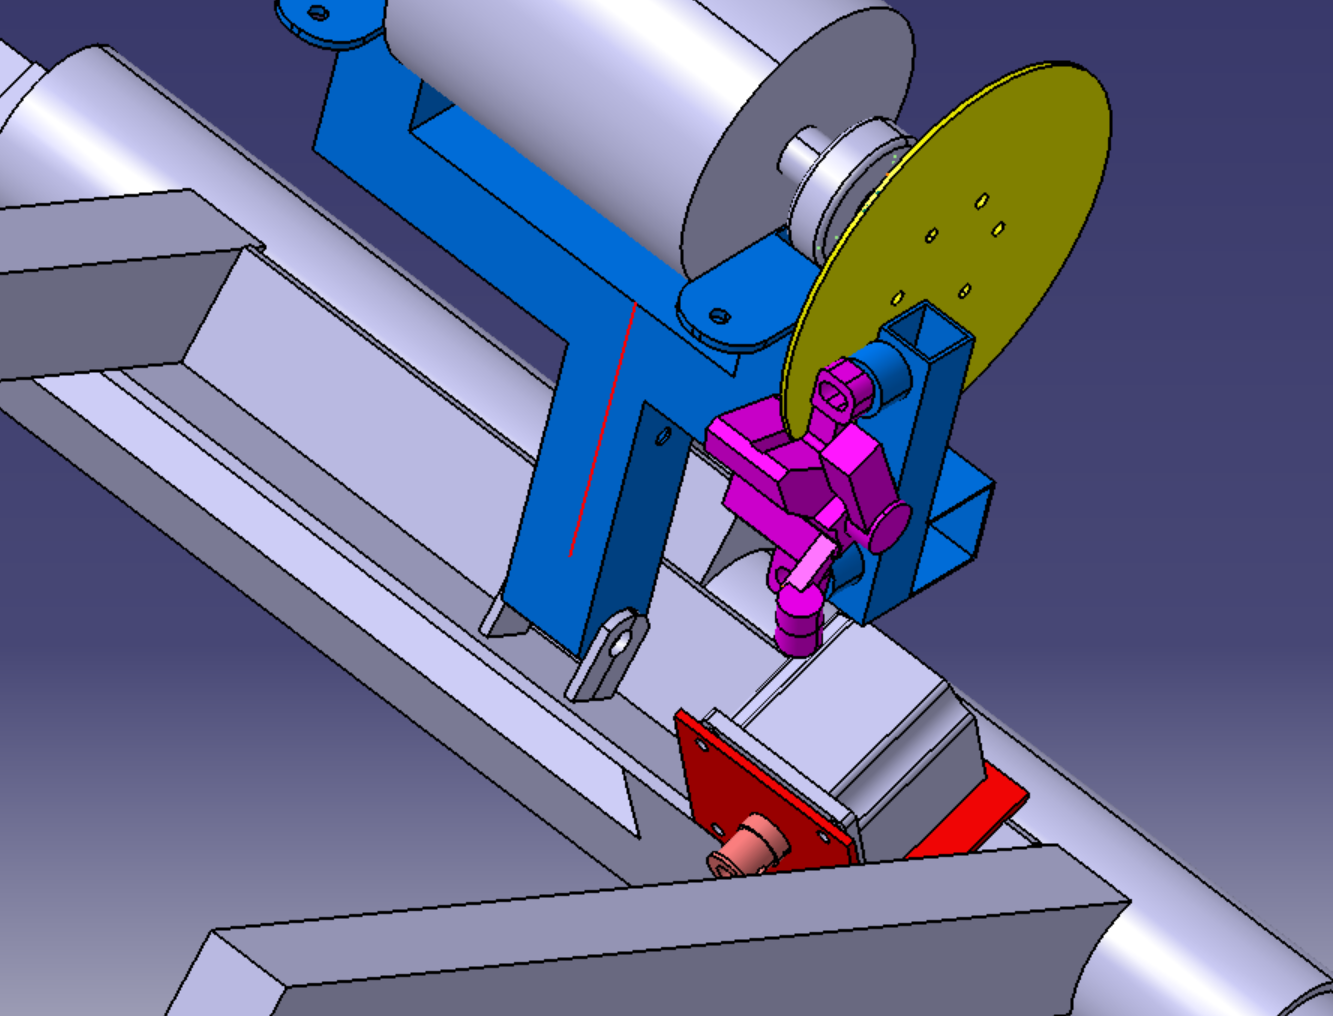
\includegraphics[scale=0.5]{figuras/carga_peso}
        \captionof{figure}{Sistema de carga de peso na simulação. Em amarelo, o disco de freio, em rosa, a pinça para frear, em vermelho o suporte do motor de passos e em azul o suporte do rolo.}
        \label{carga_peso}
    \end{center} 
    
    % Figura real do sistema de freio.

    Esta alternativa foi encontrada depois de utilização de vários iterações de simulações estruturais e CADs. Algumas coisas percebidas foram o tamanho adequado do tubo azul a ser soldado, que é ao mesmo tempo mais fácil de se fabricar quanto mais confiável no caso. As simulações de versões anteriores assim como as já apresentadas neste relatório Figuras \ref{sim_estatica_5} até \ref{vibracao_3} garantem que a estrutura aguentará os esforços.

\subsection{Alternador}
 
    Como apresentado no relatório do sistema de alimentação, o alternador não funcionou como esperado e projetado, consumindo energia ao invés de gerar. Assim, o projeto da Figura \ref{alternador} foi substituído pela utilização de um dínamo. Mais informações se encontram na sessão de energia.

    \begin{center}
        \includegraphics[scale=0.3]{figuras/alternador}
        \captionof{figure}{CAD do alternador com a correia acoplada na coroa}
        \label{alternador}
    \end{center} 
    
  \section{Integração entre áreas} \label{secao.integracao}
    
    Outra tarefa importante da equipe de estruturas foi preparar o suporte físico para sensores e motores. Para esta fase final foram concluídas tais peças, o que permitiu a integração e calibração de todo o sistema com demais sistemas.   
  
  \subsection{Suporte para medidor de velocidade}
  
  O ambiente virtual precisará saber o quão veloz esta pedalando o usuário. Isso será medido por um sensor de proximidade que mede a frequência de giro da roda. Seguindo o princípio de deixar a maior parte dos sensores no rolo, escolhemos um local de fácil montagem do sensor e fácil fabricação, o que é mostrado claramente pela figura \ref{est.sensor.prox}.
  
      \begin{center}
        \includegraphics[scale=0.5]{figuras/est_sensor_prox}
        \captionof{figure}{CAD da estrutura feita para encaixar o sensor de proximidade}
        \label{est.sensor.prox}
    \end{center} 
    
    % Foto real do suporte do sensor de proximidade
    
    Para a identificação de uma volta, foi colocado no rolo uma fita de cor diferente. Assim a cada volta o sensor identificará e o jogo saberá o quão rápido esta o usuário.
  
  \subsection{Identificação da angulação do guidão}
  
  Na parte dianteira foi feita outra adaptação na estrutura voltada para a integração com outras áreas: a mesa giratória. Por meio de um potenciômetro nela o jogo saberá qual a angulação o usuário esta aplicando no guidão.
  
       \begin{center}
        \includegraphics[scale=0.5]{figuras/est_potenciometro1}
        \captionof{figure}{CAD da mesa giratória com potenciômetro}
        \label{est.potenciometro.1}
    \end{center} 
    
    % Foto real da mesa giratória e do potenciômetro
  
  Para garantir que o potenciômetro gire juntamente com a mesa, foi feito um encaixe na mesa superior. Ainda foi feito um rasgo na mesa inferior para que se pudesse passar os fios para conectar nos computadores embarcados. Outro limitante considerado foi a angulação máxima do sensor, cerca de 270$^\circ$; foram colocados anteparos para bloquear a mesa de quebrar o equipamento. Para melhor visualização dessas características abaixo se encontra uma visão explodida da mesa giratória.
  
       \begin{center}
        \includegraphics[scale=0.5]{figuras/est_potenciometro2}
        \captionof{figure}{CAD explodido da mesa giratória com potenciômetro}
        \label{est_potenciometro2}
    \end{center} 
    
      \subsection{Controle de peso de pedalada}

  Um dos grandes desafios da parte estrutural e que foi focado desde o início, foi a preparação de um sistema que permitisse adicionar carga a pedalada para simular subidas conforme é possível se ver na sessão \ref{freio.controlado}.
  Garantir que isso fosse controlado pelo rolo era uma das prioridades, pois facilitaria a montagem da bicicleta. Com isso em mente e em constante consulta com equipe de eletrônica para entendermos todos os aspectos desse problema foi possível atingir o resultado obtido, na figura \ref{freio.completo}.
  
      \begin{center}
        \includegraphics[scale=0.5]{figuras/Freiocompleto}
        \captionof{figure}{CAD do sistema de freio para simulação de elevação}
        \label{freio.completo}
    \end{center} 
    
    % foto real do sistema de freio

    Foi feito um suporte para o motor, em vermelho, e um suporte, em salmão, para enrolar melhor o fio conectado na pinça no rolo, cujos detalhes técnicos encontram-se no anexo \ref{anexo_enrolador}.  Ainda foi feito um suporte para fixar o disco de freio no eixo do rolo, em azul claro na Figura \ref{freio.completo}, cujo desenho técnico encontra-se no anexo \ref{anexo_flange}. O fio utilizado foi de freio de bicicleta, o que garante a confiabilidade. Ainda foi soldado outra peça na parte azul para fixar a pinça. Abaixo ela é mostrada com um azul mais claro.
    
          \begin{center}
        \includegraphics[scale=0.5]{figuras/est_fixar_pinca}
        \captionof{figure}{CAD da peça de fixação da pinça}
        \label{est.fixar.pinca}
    \end{center} 